\documentclass[a4paper]{article}

\usepackage[english]{babel}
\usepackage[utf8x]{inputenc}
\usepackage{amsmath}
\usepackage{graphicx}
\usepackage[colorinlistoftodos]{todonotes}
\usepackage{hyperref}
\usepackage{listings}
\usepackage[numbers]{natbib}
\usepackage{babel,blindtext}
\usepackage{bbm}

\usepackage{algorithm}
\usepackage[noend]{algpseudocode}

\usepackage{booktabs} % To thicken table lines

\title{Learning to Trade Using Q-Learning}
\author{Uirá Caiado}

\begin{document}
\maketitle

\begin{abstract}
In this project, I will present an adaptive learning model to trade a single stock under the reinforcement learning framework. This area of machine learning consists in training an agent by reward and punishment without needing to specify the expected action. The agent learns from its experience and develops a strategy that maximizes its profits. The simulation results show initial success in bringing learning techniques to build algorithmic trading strategies.
\end{abstract}

%%%%%%%%%%%%%%%%%%%%%%%%%%%%%%%%%%%%%%%%%%%%%%%%%%%%%%%%%%%%%%%%%%%%%%%%%%%%%%%%%%%%%%%%
%% INTRODUCTION
%%%%%%%%%%%%%%%%%%%%%%%%%%%%%%%%%%%%%%%%%%%%%%%%%%%%%%%%%%%%%%%%%%%%%%%%%%%%%%%%%%%%%%%%

\section{Introduction}
\label{sec:introduction}

In this section, I will provide a high-level overview of the project, define the problem addressed and the metric used to measure the performance of the model created.

\subsection{Project Overview}
Nowadays, algo trading represents almost half of all cash equity trading in western Europe. In advanced markets, it already accounts\footnote{Source: \url{https://goo.gl/v2BENs}} for over 40\%-50\% of total volume. In Brazil its market share is not as large – currently about 10\% – but is expected to rise in the years ahead as markets and players go digital.

As automated strategies are becoming increasingly popular, building an intelligent system that can trade many times a day and adapts itself to the market conditions and still consistently makes money is a subject of keen interest of any market participant.

Given that it is hard to produce such strategy, in this project I will try to build an algorithm that just does better than a random agent, but learns by itself how to trade. To do so, I will feed my agent with one month of information about every trade and change in the top of the order book\footnote{Source: \url{https://goo.gl/k1dDYZ}} in the PETR4 - one of the most liquidity assets in Brazilian Stock Market - in a Reinforcement Learning Framework. Later on, I will test what it has learned in a newest dataset.

The dataset used in this project is also known as level I order book data\footnote{Source: \url{https://goo.gl/sP1viq}} and includes all trades and changes in the prices and total quantities at best Bid (those who wants to buy the stock) and Offer side (those who intends to sell the stock).


\subsection{Problem Statement}
Algo trading\footnote{Source: \url{http://goo.gl/b9jAqE}} strategies usually are programs that follow a predefined set of instructions to place its orders. The primary challenge to this approach is building these rules in a way that it can consistently generate profit without being too sensitive to market conditions.

Thus, the goal of this project is to develop an adaptative learning model that can learn by itself those rules and trade a particular asset using reinforcement learning framework under an environment that replays historical high-frequency data.

As \cite{chan2001electronic} described, reinforcement learning can be considered as a model-free approximation of dynamic programming. The knowledge of the underlying processes is not assumed but learned from experience.

The agent can access some information about the environment state as the order flow imbalance, the sizes of the best bid and offer and so on. At each time step $t$, It should generate some valid action, as buy stocks or insert a limit order at the Ask side. All inputs and actions will be detailed in the next sections.

The agent also should receive a reward or a penalty at each time step if it is already carrying a position from previous rounds or if it has made a trade (the cost of the operations are computed as a penalty).

Based on the rewards and penalties it gets, the agent should learn an optimal policy for trade this particular stock, maximizing the profit it receives from its actions and resulting positions.

\subsection{Metrics}
In 1988, the Wall Street Journal created a Dartboard Contest\footnote{Source: \url{http://www.automaticfinances.com/monkey-stock-picking/}}, where Journal staffers threw darts at a stock table to select their assets, while investment experts picked their own stocks. After six months, they compared the results of the two methods. After adjusting the results to risk level, they found out that the pros barely have beaten the random pickers.

Given that, the metric used to measure the performance of the learner will be the amount of money made by a random agent. So, my goal will be to outperform this agent, that should just produce some random action from a set of allowed action at each time $t$. In the next section, I will detail the behavior of this agent.

%%%%%%%%%%%%%%%%%%%%%%%%%%%%%%%%%%%%%%%%%%%%%%%%%%%%%%%%%%%%%%%%%%%%%%%%%%%%%%%%%%%%%%%%
%% ANALYSIS
%%%%%%%%%%%%%%%%%%%%%%%%%%%%%%%%%%%%%%%%%%%%%%%%%%%%%%%%%%%%%%%%%%%%%%%%%%%%%%%%%%%%%%%%

\section{Analysis}
\label{sec:analysis}

In this section, I will explore the data set that will be used in the simulation, define and justify the inputs employed in the state representation of the algorithm, explain the reinforcement learning techniques used and provide a benchmark.

\subsection{Data Exploration}
The dataset used is composed by level I order book data from PETR4, a stock traded at BMFBovespa Stock Exchange. Includes 19 trading sessions from 07/25/2016 to 08/18/2016. I will use one day to create the scalers of the features used, that I shall explain. Then, I will use 16 days to train the model and finally, I will test the policy found in the last two days. The data was collected from Bloomberg. There are 19 files, each one has 110,000 rows on average, resulting in 2,117,603 row at total and more than 86 MB of information. In the figure \ref{tab:original_data} is the stricture of one of them:

\begin{table}[ht!]
\centering
\begin{tabular}{l|llrr}
{} &                Date &   Type &  Price &   Size \\
\midrule
0 & 2016-07-25 10:02:00 &  TRADE &  11.98 &   5800 \\
1 & 2016-07-25 10:02:00 &    BID &  11.97 &   6100 \\
2 & 2016-07-25 10:02:00 &    ASK &  11.98 &  51800 \\
3 & 2016-07-25 10:02:00 &    ASK &  11.98 &  56800 \\
4 & 2016-07-25 10:02:00 &    ASK &  11.98 &  56900 \\

\end{tabular}
\caption{\label{tab:original_data}Basic Structure of the Files}
\end{table}

Each file is composed of four different fields. The column $Date$ is the timestamp of the row and has a precision of seconds. $Type$ is the kind of information that the row encompasses. The type 'TRADE' relates to an actual trade that has happened. 'BID' is related to changes in the best Bid level and 'ASK', to the best Offer level. $Price$ is the current best bid or ask and $Size$ is the cumulated quantity on that price and side.

All this data will be used to create the environment where my agent will operate. This environment is an order book, where the agent will be able to insert limit orders and execute trades at the best prices. The order book (figure \ref{tab:order_book}) is represented by two binary trees, one for the Bid and other for the Ask side. As can be seen in the table below, the nodes of these trees are sorted by price (price level) in ascending order on the Bid side and descending order on the ask side. At each price level, there are other binary trees sorted by order of arrival. The first order to arrive is the first order filled when coming in a trade.


\begin{table}[ht!]
\centering
\begin{tabular}{l|lrrl}
{} &    qBid &    Bid &    Ask &    qAsk \\
\midrule
0 &  61,400 &  12.02 &  12.03 &  13,800 \\
1 &  47,100 &  12.01 &  12.04 &  78,700 \\
2 &  51,700 &  12.00 &  12.05 &  20,400 \\
3 &  37,900 &  11.99 &  12.06 &  23,100 \\
4 &  97,000 &  11.98 &  12.07 &  27,900 \\

\end{tabular}
\caption{\label{tab:order_book}Order Book Example}
\end{table}


The environment will answer with the agent's current position and Profit and Loss (PnL) every time the agent executes a trade or has an order filled. The cost of the trade will be accounted as a penalty.

As \cite{chan2001electronic} explained, Markov decision processes (MDPs) are the most common model for reinforcement learning.  The MDP model of the environment consists, among other things, of a discrete set of states $S$ and a discrete set of actions $A$ the agent can take. About the action space $A$, there are six possibles actions:

$$a_t \in \left (None,\, buy,\, sell,\, best\_bid,\, best\_ask,\, best\_both \right)$$

Where $None$ indicates that the agent shouldn't have any order in the market. $Buy$ and $Sell$ mean that the agent should execute a market order to buy or sell $100$ stocks (the size of an order will always be a hundred shares). $best\_bid$ and $best\_ask$ indicates that the agent should keep order at the best price just in the mentioned side and $best\_both$, it should have orders at the best price in both sides.

The current state of the environment will be represented by a set of variables representing the events that have occurred at the last seconds and other variables describing the last condition of the order book. So, I will use the following inputs to represent the environment state:

\begin{itemize}
\item $log\_return$ : float. The Log return of the stock in the last 10 seconds
\item $qOFI$ : integer. The net order flow at the bid and ask in the last 10 seconds
\item $qBid$ : Integer. The size of the current best Bid
\item $book\_ratio$ : float. The Bid size over the Ask size
\end{itemize}

The size of the Ask is not used because it is indirectly used in the $book\_ratio$. The $log\_return$ is defined as $r_t = \log \left(  \frac{P_t}{P_{t-1}}\right)$, where $P_t$ is the current price and $P_{t-1}$ is the previous price. Concerning the measure of the Order Flow Imbalance (OFI), there are many ways to measure it. \cite{cont2014price} argued the *order flow imbalance* is a measure of supply/demand imbalance and defines it as a sum of individual event contribution $e_n$ over time intervals $\left[ t_{k-1}, \; t_k \right]$, such that:

$$OFI_k = \sum^{N(t_k)}_{n=N(t_{k-1})+1} e_n$$

Where $N(t_k)$ and $N(t_{k-1}) + 1$ are index of the first and last event in the interval. The $e_n$ was defined by the authors as a measure of the contribution of the $n$-th event to the size of the bid and ask queues:

$$e_n = \mathbbm{1}_{P_{n}^{B} \geq P_{n-1}^{B}} q^{B}_{n} - \mathbbm{1}_{P_{n}^{B} \leq P_{n-1}^{B}}  q^{B}_{n-1} - \mathbbm{1}_{P_{n}^{A} \leq P_{n-1}^{A}} q^{A}_{n} + \mathbbm{1}_{P_{n}^{A} \geq P_{n-1}^{A}}  q^{A}_{n-1}$$

Where $q^{B}_{n}$ and $q^{A}_{n}$ are linked to the accumulated quantities at the best bid and ask in the time $n$. The subscript $n-1$ is related to the last observation. $\mathbbm{1}$ is an indicator\footnote{Source: \url{https://en.wikipedia.org/wiki/Indicator_function}} function. In the figure below is ploted the 10-second log-return of PETR4 against the contemporaneous OFI.

\begin{figure}[ht!]
\centering
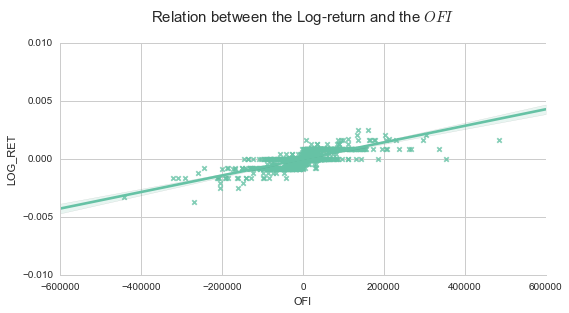
\includegraphics[width=0.75\textwidth]{figures/ofi_logret.png}
\caption{\label{fig:ofi_linear}10-second log-return against OFI}
\end{figure}

As described by \cite{cont2014price} in a similar test, the figure \ref{fig:ofi_linear} suggests that order flow imbalance is a stronger driver of high-frequency price changes and this variable will be used to describe the current state of the order book.

\subsection{Algorithms and Techniques}
Based on \cite{cont2014price}, the algo trading might be conveniently modeled in the framework of reinforcement learning. According to \cite{du1algorithm}, this framework adjusts the parameters of an agent to maximize the expected payoff or reward generated due to its actions. Therefore, the agent learns a policy that tells him the actions it must perform to achieve its best performance. This optimal policy is exactly what we hope to find when we are building an automated trading strategy.

So, defining a general formulation of the reinforcement learning problem based on a Markov Decision Process (MDP), as proposed by \cite{Mitchell}, the agent can perceive a set $S$ os distinct states of its environment and has a set $A$ of actions that it can perform. So, at each discrete time step $t$, the agent senses the current state $s_t$ and choose to take an action $a_t$. The environment responds by providing the agent a reward $r_t=r(s_t, a_t)$ and by producing the succeeding state $s_{t+1}=\delta(s_t, a_t)$. The functions $r$ and $\delta$ only depend on the current state and action (it is memoryless\footnote{Source: \url{https://en.wikipedia.org/wiki/Markov_process}}, are part of the environment and are not necessarily known to the agent.

The task of the agent is to learn a policy $\pi$ that maps each state to an action ($\pi: S \rightarrow A$), selecting its next action $a_t$ based solely on the current observed state $s_t$, that is $\pi(s_t)=a_t$. The optimal policy, or control strategy, is the one that produces the greatest possible cumulative reward over time. So, stating that:

$$V^{\pi}(s_t)= r_t + \gamma r_{t+1} + \gamma^2 r_{t+1} + ... = \sum_{i=0}^{\infty} \gamma^{i} r_{t+i}$$

Where $V^{\pi}(s_t)$ is also called the discounted cumulative reward and it represents the cumulative value achieved by following an policy $\pi$ from an initial state $s_t$ and $\gamma \in [0, 1]$ is a constant that determines the relative value of delayed versus immediate rewards. It is one of the

If we set $\gamma=0$, only immediate rewards is considered. As $\gamma \rightarrow 1$, future rewards are given greater emphasis relative to immediate reward. The optimal policy $\pi^{*}$ that will maximizes $V^{\pi}(s_t)$ for all states $s$ can be written as:

$$\pi^{*} = \underset{\pi}{\arg \max} \, V^{\pi} (s)\,\,\,\,\,, \,\, \forall s$$

However, learning $\pi^{*}: S \rightarrow A$ directly is difficult because the available training data does not provide training examples of the form $(s, a)$. Instead, as \cite{Mitchell} explained, the only available information is the sequence of immediate rewards $r(s_i, a_i)$ for $i=1,\, 2,\, 3,\,...$

So, as we are trying to maximize the cumulative rewards $V^{*}(s_t)$ for all states $s$, the agent should prefer $s_1$ over $s_2$ wherever $V^{*}(s_1) > V^{*}(s_2)$. Given that the agent must choose among actions and not states, and it isn't able to perfectly predict the immediate reward and immediate successor for every possible state-action transition, we also must learn $V^{*}$ indirectly.

To solve that, we define a function $Q(s, \, a)$ such that its value is the maximum discounted cumulative reward that can be achieved starting from state $s$ and applying action $a$ as the first action. So, we can write:

$$Q(s, \, a) = r(s, a) + \gamma V^{*}(\delta(s, a))$$

As $\delta(s, a)$ is the state resulting from applying action $a$ to state $s$ (the successor) chosen by following the optimal policy, $V^{*}$ is the cumulative value of the immediate successor state discounted by a factor $\gamma$. Thus,  what we are trying to achieve is

$$\pi^{*}(s) = \underset{a}{\arg \max} Q(s, \, a)$$

Thus, the optimal policy can be obtained even if the agent just uses the current action $a$ and state $s$ and chooses the action that maximizes $Q(s,\, a)$. Also, it is important to notice that the function above implies that the agent can select optimal actions even when it has no knowledge of the functions $r$ and $\delta$.

Lastly, according to \cite{Mitchell}, there are some conditions to ensure that the reinforcement learning converges toward an optimal policy. On a deterministic MDP, the agent must select actions in a way that it visits every possible state-action pair infinitely often. This requirement can be a problem in the environment that the agent will operate.

As the most inputs suggested in the last subsection was defined in an infinite space, in section 3 I will discretize those numbers before use them to train my agent, keeping the state space representation manageable, hopefully. We also will see how \cite{Mitchell} defined a reliable way to estimate training values for $Q$, given only a sequence of immediate rewards $r$.

\subsection{Benchmark}
As described before, the performance of my agent will be compared to the performance of a random agent. This random agent should select a random action from a set of valid action at each time step $t$.

Just like my learner, the set of action can change because the random agent is limited to hold an open position of $400$ stocks at most, on any side. When it reaches its limit, it will be allowed just to perform actions that decrease its position. So, for instance, if it already [long](https://goo.gl/GgXJgR) in $400$ shares, the possible moves would be $\left (None,\, sell,\, best\_ask \right)$. If it is [short](https://goo.gl/XFR7q3), it just can perform $\left (None,\, buy,\, best\_bid\right)$.

This performance will be measured primarily about the average reward received by the agents (that will be optimized by the learner). Later on, I will use the policy learned to simulate the learning agent behavior in a different dataset and then I will compare the final Profit and Loss and volatility of the returns of both agents. Thus, all data analyzed will be obtained by simulation.

%%%%%%%%%%%%%%%%%%%%%%%%%%%%%%%%%%%%%%%%%%%%%%%%%%%%%%%%%%%%%%%%%%%%%%%%%%%%%%%%%%%%%%%%
%% METHODOLOGY
%%%%%%%%%%%%%%%%%%%%%%%%%%%%%%%%%%%%%%%%%%%%%%%%%%%%%%%%%%%%%%%%%%%%%%%%%%%%%%%%%%%%%%%%

\section{Methodology}
\label{sec:methodology}

bla

\subsection{Data Preprocessing}
bla

\subsection{Implementation}
bla

\subsection{Refinement}
bla

%%%%%%%%%%%%%%%%%%%%%%%%%%%%%%%%%%%%%%%%%%%%%%%%%%%%%%%%%%%%%%%%%%%%%%%%%%%%%%%%%%%%%%%%
%% RESULTS
%%%%%%%%%%%%%%%%%%%%%%%%%%%%%%%%%%%%%%%%%%%%%%%%%%%%%%%%%%%%%%%%%%%%%%%%%%%%%%%%%%%%%%%%

\section{Results}
\label{sec:results}

bla

\subsection{Model Evaluation and Validation}
bla

\subsection{Justification}
bla

%%%%%%%%%%%%%%%%%%%%%%%%%%%%%%%%%%%%%%%%%%%%%%%%%%%%%%%%%%%%%%%%%%%%%%%%%%%%%%%%%%%%%%%%
%% CONCLUSION
%%%%%%%%%%%%%%%%%%%%%%%%%%%%%%%%%%%%%%%%%%%%%%%%%%%%%%%%%%%%%%%%%%%%%%%%%%%%%%%%%%%%%%%%

\section{Conclusion}
\label{sec:conclusion}

In this section, ...

\subsection{Free-Form Visualization}

bla

\subsection{Reflection}

Something really \cite{Mohri_2012}

\subsection{Improvement}

bla

%%%%%%%%%%%%%%%%%%%%%%%%%%%%%%%%%%%%%%%%%%%%%%%%%%%%%%%%%%%%%%%%%%%%%%%%%%%%%%%%%%%%%%%%
%% END
%%%%%%%%%%%%%%%%%%%%%%%%%%%%%%%%%%%%%%%%%%%%%%%%%%%%%%%%%%%%%%%%%%%%%%%%%%%%%%%%%%%%%%%%

\bibliographystyle{plain}
% or try abbrvnat or unsrtnat
\bibliography{bibliography/biblio.bib}
\end{document}
